\documentclass[11pt,aspect ratio=169]{beamer}
\usepackage{ragged2e}\justifying
\setbeamersize{text margin left=12mm, text margin right=12mm}
\setbeamertemplate{frametitle continuation}{\frametitle{\References}}
\setbeamertemplate{bibliography item}[text]
  \setbeamertemplate{enumerate items}[default]
   \setbeamercolor{item projected}{bg=white,fg=black}
\usepackage[utf8]{inputenc}
\usepackage[T1]{fontenc}
\usepackage{pdflscape}
\usepackage{booktabs}
\usepackage[numbers]{natbib}
\usepackage{bibentry}

\usepackage{lmodern}
\usepackage[english]{babel}
\usepackage{amsmath}
\usepackage{amsfonts}
\usepackage{amssymb}
\usepackage{graphicx}
\usetheme{EastLansing}
\usepackage{caption}
\usepackage{subcaption}
\usepackage{tikz}
\usetikzlibrary{arrows.meta,shapes,shadows,arrows,decorations.pathreplacing,decorations.markings}
\usepackage{subcaption}


\usepackage{smartdiagram}
%\usebeamercolor[bg]{red}
%\usecolortheme{yellow}
\usecolortheme{beaver}

\definecolor{myNewColorA}{rgb}{0,0,100}
\definecolor{myNewColorB}{rgb}{0,100,100}
\definecolor{myNewColorC}{rgb}{0,200,100}
\definecolor{myNewColorD}{rgb}{0,100,200}

\setbeamercolor*{palette primary}{bg=myNewColorA, fg = green}
\setbeamercolor*{palette secondary}{fg=darkred!70!black,bg=gray!15}
\setbeamercolor*{palette tertiary}{bg=darkred!80!black,fg=gray!10}
\setbeamercolor*{palette quaternary}{fg=darkred,bg=gray!5}
\setbeamercolor{background canvas}{bg=red!20}
\let\oldbib\bibentry
\renewcommand{\bibentry}[1]{{\tiny[\oldbib{#1}]}}
\setbeamertemplate{frametitle continuation}{\frametitle{Cont.}}
%\setbeamertemplate{frametitle continuation}{\frametitle{LITERATURE REVIEW}}

\begin{document}
	\bibliographystyle{plain}
	\nobibliography{References}
	\author{Aayushi Arya}
	  
	\title{To Theoritically model the  physical properties of a Microwave Absorber and  deriving its dielctric and magnetic parameters  for the pre selection of suitable elements and material compositions for specific microwave absorbing  applications}
		\author{\scriptsize Aayushi Arya\\
		EE18RESCH11014\\
	GUIDE Dr GVV SHARMA
\\EE Dept. IITH}

%\institute{IIT HYDERABAD}

\titlegraphic{
		\includegraphics[width=0.1\linewidth, height=0.1\textheight]{iith/IITH-LOGO}
}


%	\date{\today}
	%\subject{}
	%\setbeamercovered{transparent}
	\setbeamertemplate{navigation symbols}{}
	\begin{frame}[t]
		\maketitle
	\end{frame}
\begin{frame}
	\frametitle{Table of Contents}
	\tableofcontents
	\end{frame}
\subsection{REQUIREMENT OF MICROWAVE ABSORBERS}
	\begin{frame}[t]
		\frametitle{REQUIREMENT OF MICROWAVE ABSORBERS}
		\scriptsize
		\begin{columns}
			\column{0.6\linewidth}
		\begin{enumerate}[t]
			\item 
			\item EXPANDING COMMUNICATION INDUSTRY:With a new digital era, communication devices and speed has all shoot up, leading to large exposure to EM waves . This affects the human body ,including hearing capacity, function of enzymes and proteins(albumin protein affecting blood flow to brain) (\bibentry{pang2007densitie})
			\item ELECTROMAGNETIC INTERFERENCE : NOISE generation and signal leakage due to overlapping of the radiation noises emitted from the electronic hardware
			\item high frequency operated circuit devices like mobile phones, LAN , WIFI etc \cite{r16}.
			\item RADIATION ABSORPTION CHAMBERS FOR HIGH END EQUIPMENTSSome scientific equipments require high frequency waves to be send to characterize the sample. It has to be put in absorbing chambers
			\item RADAR and military applications : Stealth ,warships, armour coatings 
			
		\end{enumerate}
	\column{0.4\linewidth}
	\begin{figure}[l]
	
		\includegraphics[width=0.4\linewidth,height=2cm]{"C:/Users/aayushi/Documents/ALL-PHD-DOCS/latex/latex/human ear"}
		\caption{\small Effects of EM wave exposure on human ear}
		\label{fig:Effects of EM wave exposure on human ear}
	\end{figure}
	\begin{figure}[H]
		\includegraphics[width=0.7\linewidth,height=2cm]{C:/Users/aayushi/Documents/ALL-PHD-DOCS/latex/latex/EMI}
		\caption{Electro Magnetic Interference}
		\label{fig:emi}
	\end{figure}
	
		\end{columns}
	\end{frame}
\subsection{MICROWAVE ABSORBERS}
\begin{frame}{MICROWAVE ABSORBERS}
	
	\begin{columns}
	
	\column{0.5\linewidth}
	\begin{figure}[ht]
			\begin{subfigure}{0.8\textwidth}
	%	\begin{minipage}[t]{0.7\textheight}
			\includegraphics[width=0.7\linewidth]{C:/Users/aayushi/Documents/ALL-PHD-DOCS/latex/latex/EMWAVE1}
				\caption{ LAYOUT OF MA}
			\label{fig:emwave1}
	%	\end{minipage}
			\end{subfigure}
%	\end{figure}
%	\begin{figure}[H]
	%	\begin{minipage}[]{1\textheight}
			  \begin{subfigure}{0.8\textwidth}	
			\includegraphics[width=0.7\linewidth]{C:/Users/aayushi/Documents/ALL-PHD-DOCS/latex/latex/EMWAVE2}
			\caption{ELECTRICAL PARAMETERS OF MA}
			\label{fig:emwave2}
	%	\end{minipage}
			\end{subfigure}
	\end{figure}
	\column{0.5\linewidth}
%	\begin{minipage}{0.4\texwidth}
	\begin{block}{PERMITTIVITY AND PERMEABILITY}
	\begin{equation}
	\epsilon={\epsilon}^{'} +{\epsilon}^{''}
	\end{equation}
	The real part $=>$ measure of amount of energy stored in the material due to external electric field.
	The imaginary part $=>$ measure of dissipation of electrical energy.
		\begin{equation}
	\mu={\mu}^{'} +{\mu}^{''}
	\end{equation}
	The real part $=>$ measure of amount of energy stored in the material due to external magnetic field.
The imaginary part $=>$ measure of dissipation of magnetic energy.	
	\end{block}
%\end{minipage}
\end{columns}
\subsection{LITERATURE REVIEW}
\end{frame}
\begin{frame}{LITERATURE REVIEW}
	
	\begin{tabular}{p{0.4\textwidth}p{0.7\textwidth}}
	
		\toprule
		reference & Work \\
		\midrule
		\bibentry{r12} &\small Transmission Line Theory was used to model the ferrite based absorbers and find a relationship between the elctric and magnetic structure of the material to the microwave absorption. The work also shows consistency of Transmission Line Theory to the band theory of solids\\
		(\bibentry{pang2007densitie}) & \small Evaluation of  Electronic Polarizability of tranistion metals from their respective ionic radii.The changes in the ionic state of a transition metal is used to mathematically calculte the polarizabilities\\
		\bibentry{r8} & \small The mean total polarizabilities of oxides,hydroxides,oxyfluorides were emprically calculated from the free cation polarizabilities . There was application of polarizability additive rule and least square procedures,neglecting the cation coordination\\
	\bibentry{r9} & \small Lorentz-Lorenz equation was used to theoritically calculate the value of electronic and oxide ion polarizability of oxide glasses . The effect of metallization criteria was observed on the refractive index\\
		\bottomrule
	
	\end{tabular}
	\end{frame}
\subsection{PARMETER DEFINITIONS}
\begin{frame}[t,allowframebreaks]{PARMETER DEFINITIONS}
%	\begin{columns}
	%	\column[l]{0.4\linewidth}
		\small
		\begin{itemize}
			\item The existing Transmission Line Theory , which is used to analyse the microwave circuits is now being used by material scientists to evaluate different materials used as microwave absorbers. This theory has benefitted in providing an insight into the electric and magnetic parameters of Microwave Absorbers\cite{r12,r2}.
			
			%	\begin{minipage}{0.5\textwidth}{
					\begin{figure}[H]
			
				\centering
				\tiny
				\includegraphics[width=0.3\linewidth]{IMP}
				\caption{Transmission Line Schematic}
				\label{fig:imp}
					\end{figure}
			%	\end{minipage}
		%	\begin{minipage}{0.5\textwidth}
			\begin{figure}[H]
				\centering
				\includegraphics[width=0.3\linewidth]{EM3}
				\caption{Electrical and Magnetic dipolar moments\cite{r12}}
				\label{fig:em3}
			\end{figure}
			
		%	\end{minipage}
	
			
			\item Polarizability of ions(both cations and anions) is important in undersatnding the dieectric and lattice dynamical behaviour of the compounds.
			\item It can be associated with the dielectric constant and the refractive indices of a material with Lorentz=Lorenz equation
			\item Polarizability can be seen as a effect of the electronegativity of the atoms, creating a separation of positive and negative charges\cite{r10,r11}.
			\item The very basic understanding of polarizability as given by Kazimierz Fajans 1923, illustrates the effect of two oppositely charged ions on each other.When a cation which is more electropositive attracts electrons from the outer shell of the anion, thus deforming the anion.This ability of cation is called the polarisation power , the ability of anion to get polarized is called its polarizability.The factors affecting this are:
			cationic radii(higher concentration of positive charge),anionic radii(loose bound electrons),charged ions(electrostatistics).
			\item It is this deformation of ions which creates a dipole between  the positive and negative centre of charges. This deformation can be inherent or can be induced by external field creating a dipolar polarizability. Not only can it induce new dipoles, but free rotate the pre esisting dipoles to orient in a particular direction.
			\begin{figure}[H]
				\tiny
				\includegraphics[width=0.6\linewidth, height=0.2\textheight]{Dipole}
				\caption{Deformation due to polarization\cite{r11}}
				\label{fig:dipole}
			\end{figure}
			
          \item In some of the microwave absorbers , especially composite or dispersive materix based , there is \colorbox{red}{MAXWELL-WAGNER POLARIZATION} or space charge polarization ,induced by an electrical potential resulting from internal charge builds at the interfaces in a heterogenous material\cite{13}
			
			\item The relationship between molar refraction to refractive index and molar volume of a polycrystalline material is given by \textbf{Lorentz-Lorenz} equation$
			R_m = (\dfrac{n^2_o -1}{n^2_o +2 })V_m $ \cite{r9,r10}\\
			\item $R_M(m^3/mol)$ is the molar refractivity and is a measure of the total polarizability of a mole of a substance .$V_M$ is the molar volume.
			Using the same the energy gap of the compound is calculated as $E_g(eV) = 20(1- \dfrac{R_m}{V_m})^2$.This energy can be considered equivalent to the polarisation energy of an ion.
		\end{itemize}

	\begin{figure}
		%	\resizebox{0.4\textwidth}{!}{
		\tiny
		\centering
		\includegraphics[width=0.4\linewidth,height=0.4\textheight]{POL}
		\caption{DIFFERENT TYPES OF POLARIZATIONS\protect \cite{booke}}
		\label{fig:pol}
%	}
	\end{figure}

%	\end{columns}
	\end{frame}
\subsection{THEORITICAL MODELLING OF MICROWAVE ABSORPTION}
\begin{frame}{THEORITICAL MODELLING OF MICROWAVE ABSORPTION}
\begin{columns}[]
\column{0.5\textwidth}

\begin{itemize}
	\item USE OF TRANSMISSION LINE THEORY to theoritically model the resonant and non-resonant oscillation based microwave absorption.
	\item This theory , establishes the interaction of net absorption to the physical electric and magnetic parameters of the MA.
The above model is independent of underlying absorption mechanism viz. as absorption from resonance, dielectric or magnetic media , from resonance or forced non resonance oscillation.
\item GENERAL PREDICTIVE MODEL which can be used to understand the behaviour of the microwave absorbing materials.
\end{itemize}
\column{0.5\textwidth}
\begin{itemize}

\item THis theory can be used to find the influence of a variety of physical parameters and material properties arising from the atomic configurations, on their microwave absorbing characteristics.
\item This theory provides a way of deeper undersatnding into the required materislistic aspects of an ideal MA , which can lay a platform to design and explore new engineered materials for various applications
\end{itemize}

\end{columns}
\end{frame}
\subsection{TRANSMISSION LINE THEORY}

\begin{frame}[t]{TRANSMISSION LINE THEORY}
	\begin{block}{IMPEDANCE MATCHING}
For the EMI shielding applications, the prerequisite is to minimize the reflection and maximize the absorption of the incident EM wave.Keeping the Relection Loss value to be \colorbox{blue}{R.L = -20 dB}, which means that 99percenatge of microwave is absorbed, the input impedance $Zin$ at the air–material interface can be calculated as:-
\begin{equation}
RL(dB) = 20 log\mid{\dfrac{Z_{in}- Z_o}{Z_{in}+ Z_o}}\mid
\end{equation}


Using the above , we can evaluate the characteristic impedance of the microwave absorber , which is related to the intrinsic parameters of the material:-
%$$
%R.L = 20 \log(\frac{Z_o}{4Z_{in}}) \label{eq3} \\

%$$
\end{block}

\end{frame}
\subsection{FLOW CHART}
\begin{landscape}
	\begin{frame}
%\resizebox{0.5\textwidth}{!}{
%	\begin{figure}{0.8\textwidth}
	%\subfigure{
	\begin{minipage}{0.7\textwidth}
\resizebox{0.8\textwidth}{!}{
	
		
	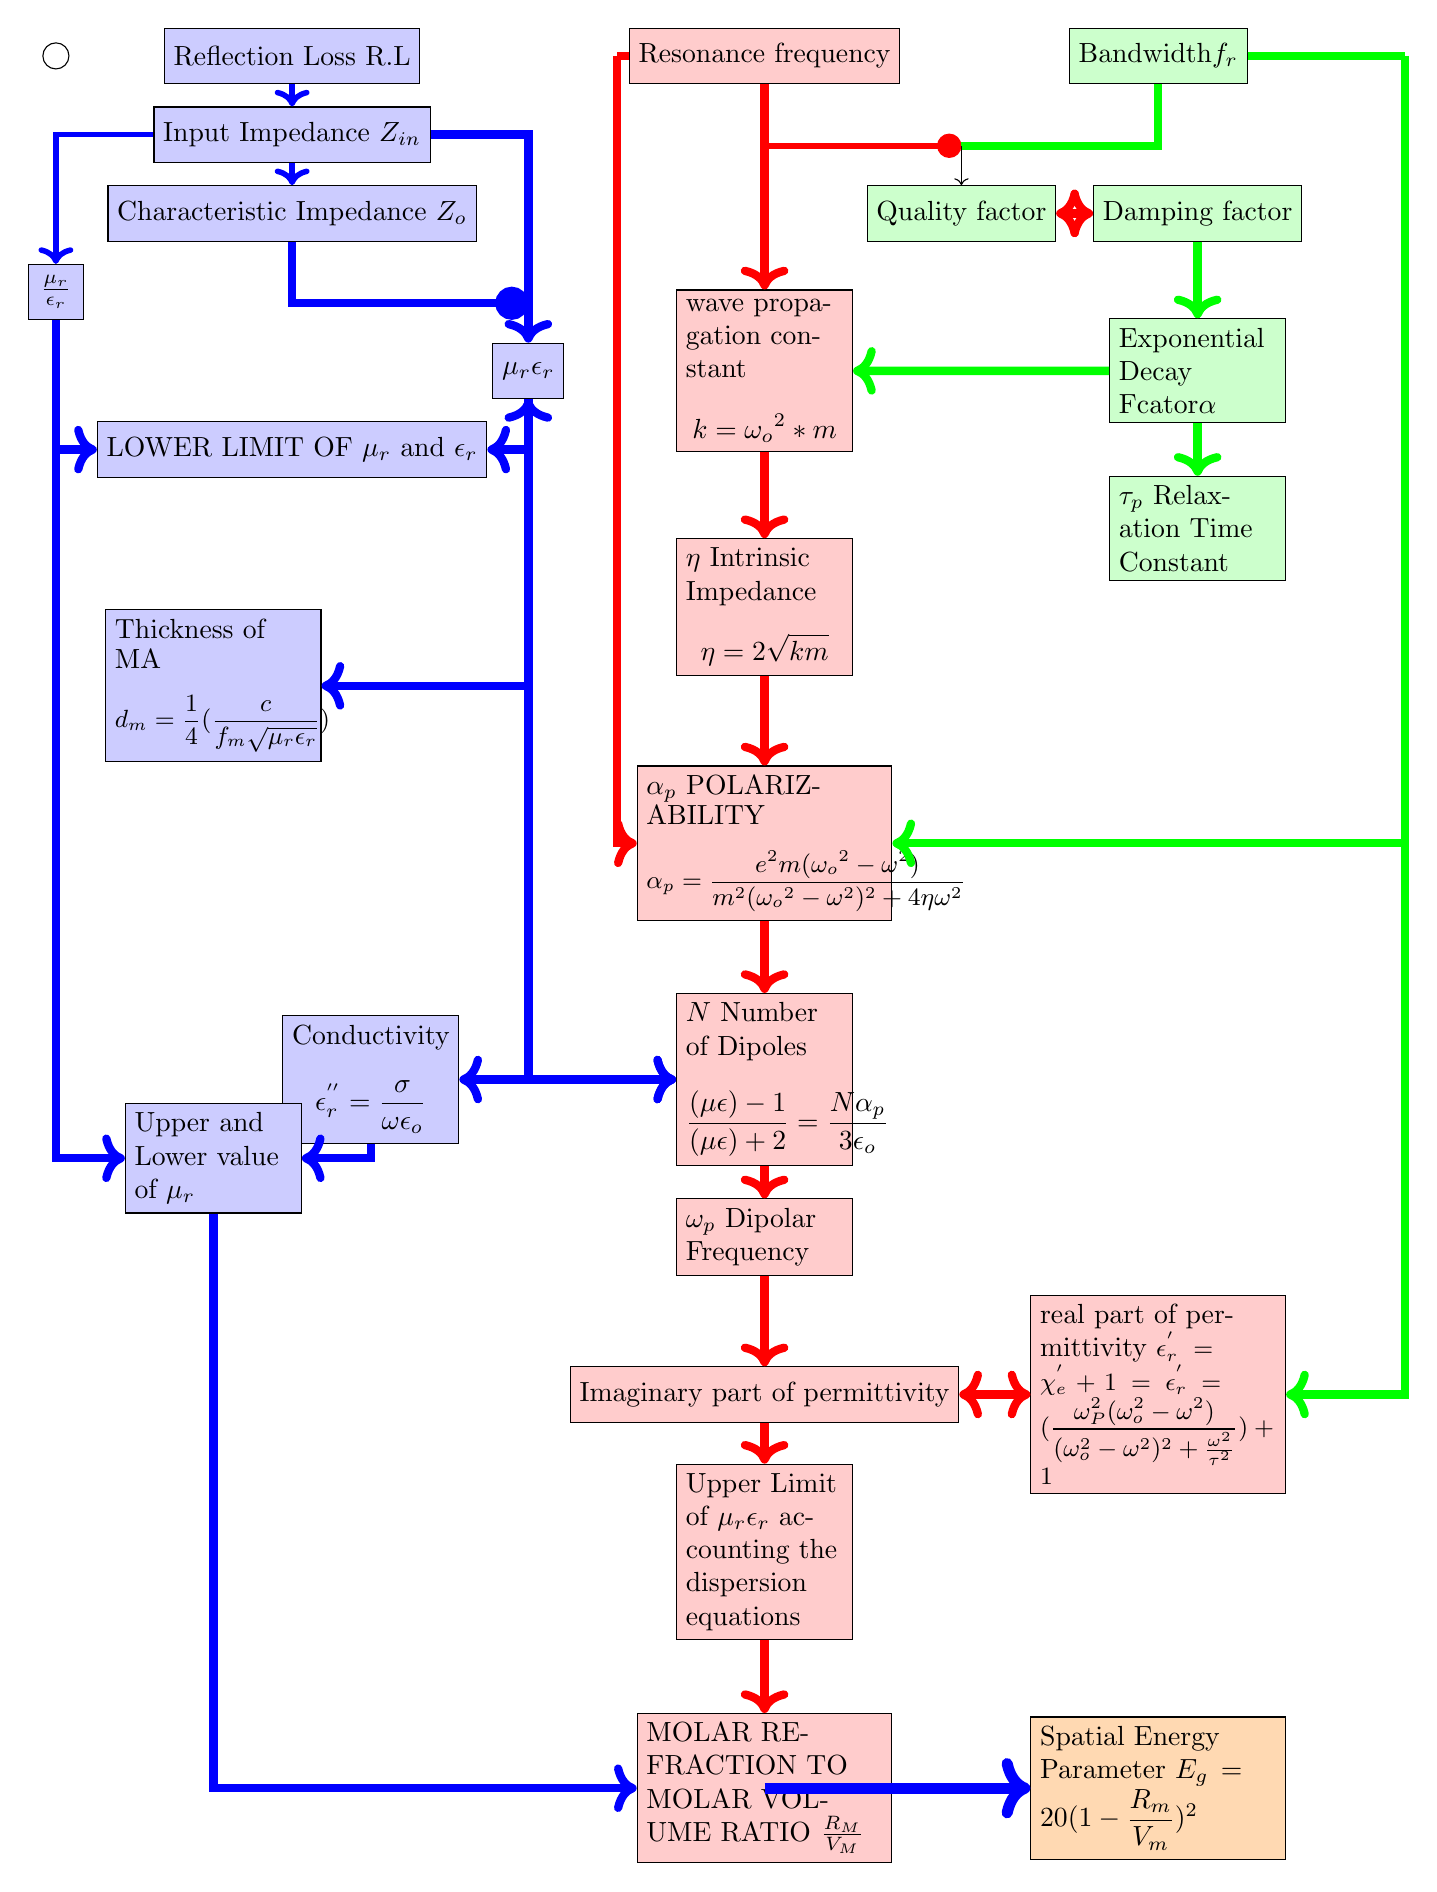
\begin{tikzpicture}
	\tikzstyle{N} = [draw,fill=blue!20,minimum size=2em,node distance=3cm]
	\tikzstyle{Nr} = [draw,fill=red!20,minimum size=2em,node distance=7cm]
	\tikzstyle{Ng} = [draw,fill=green!20,minimum size=2em,node distance=5cm]
	\def\radius{.7mm} 
	\tikzstyle{branch}=[fill,shape=circle,minimum size=3pt,inner sep=0pt]
	\node[draw,circle](o) at (0,0){};
	%\node[draw,circle,below of =F1](o) {};
	\node[N,right of=o](RL) {Reflection Loss R.L};
	%\node[N,below of=O,xshift=-5cm](RL)  {Reflection Loss R.L};
	\node[Nr,right of=RL,node distance=6cm](fo)  {Resonance frequency};
	\node[Ng,right of =fo](fr) {Bandwidth$f_r$};
	\node[N,below of=RL,node distance=1cm](Zin) {Input Impedance $Z_{in}$};
	\draw[->,line width=2pt,color=blue](RL) to (Zin);
	\node[N,below of=Zin,node distance=1cm](Zo) {Characteristic Impedance $Z_{o}$};
	\draw[->,line width=2pt,color=blue](Zin) to (Zo);
	\node[N,below of=Zo,node distance=1cm,xshift=-3cm](ratio) {$\frac{{\mu}_r}{{\epsilon}_r}$};
	\draw[->,line width=2pt,color=blue](Zin) -| (ratio);
	\node[N,below of=Zo,node distance=2cm,xshift=3cm](mult) {${\mu}_r{\epsilon}_r$};
	\draw[->,line width=3pt,color=blue](Zin) -| (mult);
	\draw[-Circle,line width=3pt,color=blue](Zo) |- ([yshift=0.5cm]mult.north);
	\node[N,below of=Zo,node distance=3cm](FD) {LOWER LIMIT OF ${\mu}_r$ and  ${\epsilon}_r$  };
	\draw[->,line width=3pt,color=blue](ratio) |- (FD);
	\draw[->,line width=3pt,color=blue](mult) |- (FD);
	\node[Ng,below of=fo,node distance=2cm,xshift=2.5cm](Q) {Quality factor};
	\draw[-Circle,line width=2pt,color=red](fo) |- ([yshift=0.5cm]Q.north);
	\draw[-,line width=3pt,color=green](fr) |- ([yshift=0.5cm]Q.north);
	\draw[->]([yshift=0.5cm]Q.north) to (Q);
	\node[Ng,right of=Q,node distance=3cm](D) {Damping factor};
	\draw[<->,line width=3pt,color=red](Q) to (D);
	%\node[Nr,below of=fo,node distance=4cm,text width=2cm](wn) {Natural Resonant Frequency${\omega}_n$};
	%\draw[->,line width=3pt,color=red](fo) to (wn);
	%\draw[-Circle,line width=3pt,color=red](Q) |- ([yshift=1cm]wn.north);
	\node[Ng,below of=D,node distance=2cm,text width=2cm](alpha) {Exponential Decay Fcator$\alpha$};
	\draw[->,line width=3pt,color=green](D) to (alpha);
	\node[Nr,below of=fo,node distance=4cm,text width=2cm](k) {wave propagation constant$$k = {\omega_o}^2*m$$};
	\draw[->,line width=3pt,color=green](alpha) to (k);
	
	%\draw[->,line width=3pt,color=red](wn) to (k);
	\node[Nr,below of =k,node distance=3cm,text width=2cm](n) {$\eta$ Intrinsic Impedance$$\eta = 2 \sqrt{km}$$};
	\draw[->,line width=3pt,color=red](k) to (n);
	\node[Nr,below of =n,node distance=3cm,text width=3cm](ap) {${\alpha}_p$ POLARIZABILITY\small{$${\alpha}_p = \dfrac{e^2 m ({\omega_o}^2 - {\omega}^2)}{m^2({\omega_o}^2 - {\omega}^2)^2 + 4 \eta \omega^2} $$}};
	\draw[->,line width=3pt,color=red](n) to (ap);
	\node[Nr,below of =ap,node distance=3cm,text width=2cm](nd) {$N$ Number of Dipoles$$\dfrac{({\mu \epsilon})- 1}{({\mu \epsilon}) + 2 } = \dfrac{N \alpha_p}{3 \epsilon_o}$$};
	\draw[->,line width=3pt,color=red](ap) to (nd);
	\node[Nr,below of =nd,node distance=2cm,text width=2cm](wp)  {${\omega}_p$ Dipolar Frequency};
	\draw[->,line width=3pt,color=red](nd) to (wp);
	\draw[->,line width=3pt,color=red](fo) to (k);
	\draw[-,line width=3pt,color=red](fo.west) to ([xshift=2.5cm]RL.east);
	\draw[->,line width=3pt,color=red]([xshift=2.5cm]RL.east) |- (ap) ;
	\node[Ng,below of =alpha,node distance=2cm,text width=2cm](tc) {${\tau}_p$ Relaxation Time Constant};
	\draw[->,line width=3pt,color=green](alpha) to (tc);
	\draw[->,line width=3pt,color=blue](mult) |- (nd);
	
	\node[Nr,below of =wp,node distance=2cm](im) { Imaginary part of permittivity};
	
	%\node[Nr,below of =im,node distance=2cm,text width=2cm](re) {real part of permittivity};
	\draw[-,line width=3pt,color=green](fr.east) to ([xshift=2cm]fr.east);
	\draw[->,line width=3pt,color=green] ([xshift=2cm]fr.east) |- (ap);
	%\draw[-,line width=3pt,color=blue](wp) to ([yshift=0.5cm]wp.south);
	\node[N,below of =FD,xshift=-1cm,node distance=3cm,text width=2.5cm](d) { Thickness of MA\small{ $$d_m = \frac{1}{4}(\frac{c}{f_m \sqrt{\mu_r \epsilon_r}}) $$}};
	\draw[<->,line width=3pt,color=blue] (d.east) -| (mult);
	\node[N,left of =nd,node distance=5cm,text width=2cm](sig) { Conductivity $$\epsilon^{''}_r = \dfrac{\sigma}{\omega \epsilon_o} $$};
	\draw[<->,line width=3pt,color=blue] (sig) to (nd);
	\node[Nr,right of =im,node distance=5cm,text width=3cm](re) { real part of permittivity\small{ 
			$\epsilon^{'}_{r } = \chi^{'}_{e} + 1 =
			\epsilon^{'}_r = (\dfrac{\omega^2_P (\omega^2_o - \omega^2)}{(\omega^2_o - \omega^2)^2 + \frac{\omega^2}{\tau^2}}) + 1 $}};
	\draw[-,line width=3pt,color=green](fr.east) to ([xshift=2cm]fr.east);
	\draw[->,line width=3pt,color=green] ([xshift=2cm]fr.east) |- (re);
	\draw[->,line width=3pt,color=red] (wp) to (im);
	\draw[<->,line width=3pt,color=red] (im) to (re);
	\node[Nr,below of =im,node distance=2cm,text width=2cm](FU) {Upper Limit of $\mu_r \epsilon_r$ accounting the dispersion equations};
	\draw[->,line width=3pt,color=red] (im) to (FU);
	\node[N,below of =d,node distance=6cm,text width=2cm](pm) {Upper and Lower value of $\mu_r $};
	\draw[->,line width=3pt,color=blue] (ratio) |- (pm);
	\draw[->,line width=3pt,color=blue] (sig) |- (pm);
	\node[Nr,below of =FU,node distance=3cm,text width=3cm](RV) {MOLAR REFRACTION TO MOLAR VOLUME RATIO $\frac{R_M}{V_M}$};
	\draw[->,line width=3pt,color=red] (FU) to (RV);
	\draw[->,line width=3pt,color=blue] (pm) |- (RV);
	\node[N,fill=orange!30,right of =RV,node distance=5cm,text width=3cm](Eg) {Spatial Energy Parameter $E_g = 20(1- \dfrac{R_m}{V_m})^2$};
	\draw[->,line width=4pt,color=blue] (RV) |- (Eg);
	\end{tikzpicture}
}
	%\end{subfigure}
	\end{minipage}
	%}
	%\end{figure}
%}
\end{frame}
\end{landscape}
\subsection{ATOMIC PARAMETERS}
\begin{frame}[t]{ATOMIC PARAMETERS}
	\scriptsize
The polarisation Energy will be calculated using	the principle of adding inverse values of volume energies and kinetic parameters whcih has been used in many different physical and chemical processes.
Since Polarisation can be related to the force exerted by the valence electrons that is the electron affinity,and their inertness to form direct bond that is the ionization potential, screened through nucleus charges,it can be calculated proportionally via the inverse addition of orbital energy (accounting for the attraction or repulsion by electrons) and the effective nucleus energy.
$$\dfrac{1}{{q^2}} + \dfrac{1}{\eta} = \dfrac{1}{P_o}$$
where $\eta$ is the global hardness factor
$q=\frac{z^{*}}{n^{*}}$, $z^{*}$ is the effective charge of nucleus and $n^{*}$ is the effective main quantum number.
\colorbox{red}{$P_o (eV \AA)$ is called the spatial energy parameter} and \colorbox{red}{$P_E(eV \AA)$} is called the effective P-parameter for polarization.$P_E$ is a physical parameter , accounting for the averaged polarisation energy over the valence electrons.
$\eta$ is the global hardness factor , which is calculated from the ionization potential and the electron affinity of the atom. By considering the simple electrostatic coulumbic forces across atoms,it can also be calculated as $\eta=\frac{e^2}{2R}$.
\\


	\end{frame}
\begin{frame}[t]
	Effective principal quantum number can be calculated as a cumulative effect of the orbiatl exponent value $\xi$ of each shell occupied, the outer shell value and the average spin of the outer shell. 
	\\
	Effective principal quantum number    =\hspace{2cm} orbital exponents of each shell (taking effect of screening charges)
	
	%\noindent\rule[0.5ex]{0.5\linewidth}{1pt}
	\hspace{6cm}\noindent\rule{10cm}{0.4pt}\\
	\hspace{6cm}outer shell Orbital exponent*outer shell quantum number*average spin
	\\
	Similarlt the \colorbox{red}{effective nucleus charge $q (eV \AA)$},  can be calculated from the nucleus charge minus the screening effect.
	
	The last parmeter that is $P_E$ can be calculated as $$P_E = \frac{P_o}{r_i}$$,where $r_i (\AA)$ is the atomic radii of atom.
	The effective polaristaion parameter can be used for comparing the suitability of different elements in different material compositions for the Microwave Absorbing Applications.
	\bibentry{r1}
	\end{frame}
\subsection{MATERIALS}
\begin{frame}{MATERIALS}
	\begin{columns}[T]
		\column{0.6\textwidth}
	\begin{itemize}
		\scriptsize
		\item \colorbox{green}{METALLIC PERVOSKITE MATERIAL} Benefits of using pervoskite is broad EM wave absorption spectrum, environment stability, chemically inert,unique physical properties for metallic ground states,balance between permittivity and peremability\cite{13}.
		\item Pervoskite materials have already been established as a microwave dielectric used in wireless communication devices viz. resonators,filters, temperature stable capacitor as shown in figure.
		\item These materials , which have been studied for more than a half century, shows immense potential as microwave absorbers owing to its resonating dielectric polarization across its cryatal structure Some examples include$LaNiO_3$,.
		\item \colorbox{green}{HIGH ENTROPY OXIDES} HEOs are new engineered materials that have a multi cationic configuration , leading up to an increase in the entropy of the compound. The entropy stabalization imparts them functional properties(more stable dielectric behaviour).These  properties can be engineered with much flexibility. Examples are $(Co_{0.2} Cu_{0.2} Mg_{0.2} Ni_{0.2} Zn_{0.2})O_3$ \cite{r15}
			\end{itemize}
		\column{0.5\textwidth}
		\begin{figure}[H]
			\centering
			\includegraphics[width=0.7\linewidth]{mat}
			\caption{microwave dielectrics \protect \cite{r14}}
			\label{fig:mat}
		\end{figure}
		
	\end{columns}
	\end{frame}

\begin{frame}[t]{MATERIALS}
	\begin{itemize}
		\item \colorbox{green}{FERRITES} Ferrites have found popularity as Microwave Absorbers owing to the magnetic losses along with dielctric losses giving high absorption at wide frequency range.Impedance matching of Ferrite is more improved than pure dielectrics because of low eddy current loss\cite{r18}.
		\item X-type HEXAGONAL FERRITES, with high saturation magnetization, low coercivity, excellent chemical stability serve as good microwave absorbers.
		\item RARE EARTH elements have certain relaxation properties which enhances the EM wave properties of ferrites\cite{r16}.
		\item MANGANITE MATERIALS manganites like $La_{0.8}Ca_{0.2-x}Ag_x Mn O_3$ (x=0.05 to 0.15) have shown good microwave absorption propeties as shown in \cite{r17,r18}
		\item \colorbox{green}{RARE EARTH doped OXIDES} rare earth doped oxides have shown better microwave absorption properties with wide peak behaviour. The dynamic behaviour of compound changes with rare earth doping \cite{r19}
	\end{itemize}
	\end{frame}
\subsection{MAGNETIC PARAMETERS}
\begin{frame}[t]{MAGNETIC PARAMETERS}
\begin{tabular}{p{0.2\textwidth}p{0.4\textwidth}p{0.4\textwidth}}
	S.No & d-shell & f-shell\\
	\hline
Real Part of Permeability & $\mu^{'}$ & $\mu^{'}$\\
	\hline
Imaginary part of Permeability & $\mu^{''} = \dfrac{c}{2 \pi d f_m}$ & $\mu^{''} = \dfrac{2 \pi \mu_o {(\mu^{'})}^2 \sigma \delta^{2} f}{3}$\\
	\hline
Suscpetibility & Atomic Susceptibilty $\chi_A$ & Molar Susceptibilty $\chi_M$
	
	\\
	\hline
	
Magnetic Dipole Moment & Spin Magnetic Dipole Moment $$\mu_s = 2.84 \sqrt{\chi_A T} B.M$$ & Orbital angular moment$$\mu_{J} = {[\dfrac{3kT\chi_A}{N {\mu_B}^2}]}^{1/2}$$
	\\
\end{tabular}

	\end{frame}

%\end{frame}
%\begin{frame}[t,allowframebreaks]{References}
%	\begin{thebibliography}{9}
%		\tiny
%		\bibitem{1}SHANKER1977359,
%		title = "Electronic polarizabilities of ions in transition metal oxides",
%		journal = "Solid State Communications",
%		volume = "21",
%		number = "4",
%		pages = "359 - 361",
%		year = "1977",
%		issn = "0038-1098",
%		doi = "https://doi.org/10.1016/0038-1098(77)91245-5",
%		url = "http://www.sciencedirect.com/science/article/pii/0038109877912455",
%		author = "Jai Shanker and H.P. Sharma and B.R.K. Gupta"
%	\end{thebibliography}
%\end{frame}

%\begin{frame}[allowframebreaks]{References}
\bibliographystyle{unsrt}
\nobibliography{References.bib}
%\end{frame}
\begin{frame}[allowframebreaks]{References}
	\begin{enumerate}
	
\item
	Review of electromagnetic interference shielding materials fabricated by iron ingredients,Shukla, Vineeta,
	Nannoscale Advances,vol 1,
	no.5,
	p. 1640-1671,
	2019,Royal Society of Chemistry


\item
	A theoretical and practical clarification on the calculation of reflection loss for microwave absorbing materials,
	Liu, Ying and Zhao, Kun and Drew, Michael GB and Liu, Yue,AIP Advances,
	vol 8,
	no.1,
	p. 015223, 2018, AIP Publishing LLC


\item
	Bandwidth, Q factor, and resonance models of antennas,
	Gustafsson, Mats and Nordebo, Sven,
	journal={Progress in Electromagnetics Research},
	vol 62,
	p.1-20, 2006,EMW Publishing

\item
	Frequency Response: Resonance, Bandwidth, Q Factor,
	Cory, David and Manos, C, URL https://ocw. mit. edu/courses/electrical-engineering-and-computer-science/6-071j-introduction-to-electronics-signals-and-measurement-spring-2006/lecture-notes/resonance $\{$\_$\}$ qfactr. pdf, 2006

\item
	Electronic circuits: fundamentals and applications,
	Tooley, Mike,2019, Routledge,
	p.77-78

\item
	Quality Factor / Q Factor; formulas and equations,Ian Poole
	2016,
	Accessed on :Dec. 15 2019,
	howpublished Online,
	url https://www.electronics-notes.com/articles/basic concepts/q-quality-factor/basics-tutorial-formula.php

\item
	Metamaterial: Smart Magnetic Material for Microwave Absorbing Material,Adi, Wisnu and Yunasfi, Yunasfi and Mashadi, Mashadi and Winatapura, Didin and Mulyawan, Ade and Sarwanto, Yosef and Gunanto, Yohanes and Taryana, Yana
     02,2019,
	10.5772/intechopen.84471

\item 
Empirical electronic polarizabilities in oxides, hydroxides, oxyfluorides, and oxychlorides,
Shannon, Robert D and Fischer, Reinhard X,
Physical Review B,	vol 73,	no. 23,	p. 235111,2006,	APS.

\item
 Polarizability and optical basicity of Er3+ ions doped tellurite based glasses,
	Azlan, MN and Halimah, MK and Shafinas, SZ and Daud, WM,
Chalcogenide Le,	vol. 11,	no. 7,	p. 319-335,	2014.

\item
 The Estimation of the Oxide Ion Polarizability for B 2 O 3-Li 2 O-Mo Glass System,Moustafa, El-Sayed and Elkhateb, Farid,
American Journal of Applied Sciences,vol. 9,	no. 3,	p. 446,
2012

\item
 Interactions involving the polarization of molecules,
Israelachvili, JN,
Intermolecular and Surface Forces,
p. 91-106,2011,	Academic Press San Diego

\item Several theoretical perspectives of ferrite-based materials—Part 1: transmission line theory and microwave absorption,	Liu, Ying and Tai, Rui and Drew, Michael GB and Liu, Yue,Journal of Superconductivity and Novel Magnetism,
	vol. 30,2489-2504,2017,
	Springer

\item
 Electromagnetic wave absorption and dielectric-modulation of metallic perovskite lanthanum nickel oxide,Jiang, JJ and Li, D and Li, SJ and Wang, ZH and Wang, Y and He, J and Liu, W and Zhang, ZD, RSC Advances,5,19,
14584-14591,2015,Royal Society of Chemistry

\item Microwave Dielectrics with Perovskite-Type Structure,
Hitoshi Ohsato,
perovskite-materials-synthesis-characterisation-properties-and-applications,5,2016,Intech Open

\item High-entropy oxides: fundamental aspects and electrochemical properties,Sarkar, Abhishek and Wang, Qingsong and Schiele, Alexander and Chellali, Mohammed Reda and Bhattacharya, Subramshu S and Wang, Di and Brezesinski, Torsten and Hahn, Horst and Velasco, Leonardo and Breitung, Ben,Advanced Materials,
	vol. 31,
	no 21,
	p. 1806236,
	2019,
	Wiley Online Library

\item Structural, infrared, magnetic and microwave absorption properties of rare earth doped X-type hexagonal nanoferrites,Sadiq, Imran and Khan, Imran and Rebrov, Evgeny V and Ashiq, Muhammad Naeem and Naseem, Shahzad and Rana, MU,Journal of alloys and compounds,
	vol. 570,
	p. 7-13,2013,Elsevier
	
	
\item   Microwave absorption properties of La0. 8Ca0. 2-xAgxMnO3 (x= 0.05; x= 0.15) synthesized by sol-gel method,
	Kurniawan, Budhy and Laksmi, W and Sahara, NA,
	Journal of Physics: Conference Series,
	vol. 1011,
	no. 1,
	p. 012008,
	2018,
	IOP Publishing.
	
\item The initial susceptibility of ferrites: A quantitative theory,Bouchaud, JP and Zerah, PG, Journal of applied physics,
	vol. 67,
	n. 9,
	p. 5512-5514,
	1990,American Institute of Physics

\item 
Chemical processing and microwave characteristics of (Zr, Sn) TiO4 microwave dielectrics",Hirano, Shin-ichi and Hayashi, Takashi and Hattori, Akiyoshi,Journal of the American Ceramic Society,
	vol. 74,
	p. 1320-1324,
	1991,
	Wiley Online Library
	
\item Electrostatics of Dielectric Materials,
	bookTitle"Basic Electromagnetism and Materials,
	2007,
	Springer New York,
p 39-87
%Available="https://doi.org/10.1007/978-0-387-49368-8_2"
\end{enumerate}
\end{frame}
\end{document}